% =====================================================================
%  Lab 6 -- Project Planning, Prioritization, Risk Management,
%           and Simple Docker Deployment
%  Chosen project: Smart Event Management Platform
% =====================================================================
\documentclass[11pt,a4paper]{article}
% =====================================================================
%  ZoneSense lab reports -- shared preamble
%  CS3151 Software Engineering, Effat University, Fall 2026
%  Compiler: pdfLaTeX (Overleaf default)
% =====================================================================

% ---------- Fonts and encoding ----------
\usepackage[T1]{fontenc}
\usepackage[utf8]{inputenc}
\usepackage{lmodern}               % Latin Modern for typewriter text
\usepackage{mathptmx}              % Times for body text
\usepackage[scaled=0.90]{helvet}   % Helvetica for table headers and captions
\usepackage{textcomp}
\usepackage{amssymb}
\usepackage{microtype}

% ---------- Page layout ----------
\usepackage[a4paper,top=2.2cm,bottom=2.2cm,left=2.2cm,right=2.2cm,headheight=16pt]{geometry}
\setlength{\parindent}{0pt}
\setlength{\parskip}{6pt plus 1pt}
\linespread{1.08}
\setlength{\emergencystretch}{2em}

% ---------- Colours (taken from the SRS) ----------
\usepackage[table]{xcolor}
\definecolor{znavy}{HTML}{173A5E}   % headings, table headers
\definecolor{zteal}{HTML}{1A9EAD}   % sub-headings
\definecolor{zrow}{HTML}{F0F5FA}    % alternating table rows
\definecolor{zline}{HTML}{B7C6D5}   % table rules
\definecolor{znote}{HTML}{FFF6DB}   % call-out background
\definecolor{znotebar}{HTML}{D9A21B}% call-out bar
\definecolor{zpink}{HTML}{FBEDED}
\definecolor{zmint}{HTML}{E3F4F1}
\definecolor{zgreen}{HTML}{1E7B3A}
\definecolor{zcode}{HTML}{F5F7F9}

% ---------- Packages ----------
\usepackage{graphicx}
\usepackage{array}
\usepackage{tabularx}
\usepackage{xltabular}
\usepackage{makecell}
\usepackage{enumitem}
\usepackage{titlesec}
\usepackage{fancyhdr}
\usepackage{float}
\usepackage{caption}
\usepackage{needspace}
\usepackage[most]{tcolorbox}
\usepackage{listings}
\usepackage{xurl}
\usepackage[hidelinks]{hyperref}
\urlstyle{same}

\graphicspath{{figures/}}

% ---------- Headings ----------
\setcounter{secnumdepth}{3}
\titleformat{\section}{\LARGE\bfseries\color{znavy}}{\thesection.}{0.5em}{}
\titleformat{\subsection}{\Large\bfseries\color{zteal}}{\thesubsection}{0.6em}{}
\titleformat{\subsubsection}{\large\bfseries\color{znavy}}{\thesubsubsection}{0.6em}{}
\titleformat{\paragraph}[runin]{\normalsize\bfseries\color{znavy}}{}{0pt}{}
\titlespacing*{\section}{0pt}{6pt}{12pt}
\titlespacing*{\subsection}{0pt}{14pt}{6pt}
\titlespacing*{\subsubsection}{0pt}{12pt}{4pt}
\titlespacing*{\paragraph}{0pt}{8pt}{0.6em}

% ---------- Lists ----------
\setlist{itemsep=2pt,topsep=3pt,parsep=0pt}

% ---------- Tables ----------
\newcolumntype{L}[1]{>{\raggedright\arraybackslash}p{#1}}
\newcolumntype{C}[1]{>{\centering\arraybackslash}p{#1}}
\newcolumntype{Y}{>{\raggedright\arraybackslash}X}
\newcolumntype{B}[1]{>{\raggedright\arraybackslash\leavevmode\bfseries\color{znavy}}p{#1}} % bold navy first column
\newcolumntype{Z}{>{\centering\arraybackslash}X}
\renewcommand{\arraystretch}{1.25}
\setlength{\tabcolsep}{5pt}
\arrayrulecolor{zline}
\newcommand{\hd}[1]{\leavevmode\textcolor{white}{\sffamily\bfseries #1}}   % header cell
\newcommand{\headrow}{\rowcolor{znavy}}                            % header row
\newcommand{\stripe}{\rowcolors{2}{white}{zrow}}                    % zebra rows

% ---------- Captions ----------
\captionsetup{font={small,sf},labelfont={bf,color=znavy},textfont={bf,color=znavy},
  labelsep=endash,justification=raggedright,singlelinecheck=false,skip=4pt}
\captionsetup[figure]{font={small,sf},labelfont={color=gray},textfont={color=gray},
  justification=centering,singlelinecheck=true,skip=6pt}

% ---------- Handy macros ----------
\newcommand{\COtwo}{CO\textsubscript{2}}
\newcommand{\tick}{\ensuremath{\checkmark}}
\newcommand{\gtick}{\textcolor{zgreen}{\ensuremath{\checkmark}}}
\newcommand{\cbox}{\ensuremath{\square}}

% Call-out box (yellow, left bar) -- used for notes in the SRS
\newtcolorbox{zcallout}{enhanced,breakable,colback=znote,colframe=znote,
  borderline west={3pt}{0pt}{znotebar},arc=0pt,outer arc=0pt,
  left=8pt,right=8pt,top=5pt,bottom=5pt,fontupper=\small,before skip=8pt,after skip=8pt}

% Light-blue information box
\newtcolorbox{zinfo}{enhanced,colback=zrow,colframe=zrow,arc=0pt,outer arc=0pt,
  left=8pt,right=8pt,top=6pt,bottom=6pt,fontupper=\small,before skip=8pt,after skip=8pt}

% Code listings
\lstset{basicstyle=\ttfamily\scriptsize,columns=fullflexible,keepspaces=true,
  breaklines=true,breakatwhitespace=false,showstringspaces=false,upquote=true,
  frame=single,rulecolor=\color{zline},backgroundcolor=\color{zcode},
  xleftmargin=4pt,xrightmargin=4pt,framexleftmargin=4pt,framexrightmargin=4pt,
  aboveskip=8pt,belowskip=8pt,tabsize=4,
  literate={≤}{{$\le$}}1 {≥}{{$\ge$}}1 {→}{{$\rightarrow$}}1 {–}{{--}}1}

% ---------- Header and footer ----------
\pagestyle{fancy}
\fancyhf{}
\fancyhead[L]{\small\sffamily\textcolor{znavy}{\ShortTitle}}
\fancyhead[R]{\small\sffamily\textcolor{gray}{CS3151 -- Software Engineering}}
\fancyfoot[L]{\footnotesize\sffamily\textcolor{gray}{CS3151/2026 \quad Dr.\ Passent Elkafrawy}}
\fancyfoot[R]{\footnotesize\sffamily\textcolor{gray}{\thepage}}
\renewcommand{\headrulewidth}{0.4pt}
\renewcommand{\headrule}{\hbox to\headwidth{\color{zline}\leaders\hrule height \headrulewidth\hfill}}

% ---------- Cover page ----------
% Set \LabTitle, \ProjectTitle and \TeamMembers in main.tex before \begin{document}.
\newcommand{\makecover}{%
  \begin{titlepage}
    \centering
    \vspace*{1.2cm}
    
\includegraphics[width=3.6cm]{effat_logo.png}\par
    \vspace{1.6cm}
    {\Large\bfseries Course: CS3151 -- Software Engineering\par}
    \vspace{0.35cm}
    {\large\bfseries Project -- Fall 2026\par}
    \vspace{0.15cm}
    {\large\bfseries Instructor: Dr.\ Passent Elkafrawy\par}
    \vspace{1.6cm}
    {\large\bfseries \ProjectTitle\par}
    \vspace{0.9cm}
    {\color{znavy}\rule{0.55\linewidth}{0.6pt}\par}
    \vspace{0.45cm}
    {\LARGE\bfseries\color{znavy} \LabTitle\par}
    \vspace{0.35cm}
    {\color{znavy}\rule{0.55\linewidth}{0.6pt}\par}
    \vfill
    {\large\bfseries Done By:\par}
    \vspace{0.4cm}
    {\large \TeamMembers\par}
    \vspace{2.2cm}
  \end{titlepage}%
}

% Keep a run-in heading together with the text that follows it
\newcommand{\keephead}[1]{\needspace{6\baselineskip}\paragraph{#1}\leavevmode\par\vspace{-\parskip}}

% Never leave a heading stranded at the bottom of a page
\usepackage{etoolbox}
\pretocmd{\section}{\needspace{8\baselineskip}}{}{}
\pretocmd{\subsection}{\needspace{6\baselineskip}}{}{}
\pretocmd{\subsubsection}{\needspace{5\baselineskip}}{}{}


\newcommand{\ShortTitle}{Lab 6: Project Management}
\newcommand{\LabTitle}{Lab 6: Project Planning, Prioritization,\\Risk Management, and Simple Docker Deployment}
\newcommand{\ProjectTitle}{Smart Event Management Platform}
\newcommand{\TeamMembers}{%
  Remas Rawas --- ID: S24109161\\[6pt]
  Bayan Abduldaym --- ID: S24109196\\[6pt]
  Ghala Bin Salim --- ID: S24109159\\[6pt]
  Fatima Abbas}

\newcommand{\code}[1]{\texttt{#1}}
\newcommand{\hlt}[1]{\colorbox{yellow!45}{\strut #1}}

% Lab parts and sub-headings
\newcommand{\labpart}[1]{\section*{#1}\addcontentsline{toc}{section}{#1}}
\newcommand{\labsub}[1]{\subsection*{#1}}

% Answer box
\newtcolorbox{answerbox}{enhanced,breakable,colback=zrow,colframe=zrow,
  borderline west={2.5pt}{0pt}{zteal},arc=0pt,outer arc=0pt,
  left=8pt,right=8pt,top=4pt,bottom=4pt,before skip=3pt,after skip=9pt,
  fontupper=\small\color{znavy}}
\newcommand{\answer}[1]{\begin{answerbox}\textbf{\color{zteal}Answer:} #1\end{answerbox}}

% Question line
\newcommand{\question}[1]{\needspace{4\baselineskip}\noindent #1\par}

% Python listing with syntax colours (used for app.py)
\lstdefinestyle{py}{language=Python,keywordstyle=\color{violet},stringstyle=\color{zgreen},
  commentstyle=\color{gray}\itshape,basicstyle=\ttfamily\small}
\lstdefinestyle{plain}{basicstyle=\ttfamily\small}

% Simple table (navy header, zebra rows)
\newcommand{\simplehead}[1]{\hline\headrow #1\\\hline}

\begin{document}
\makecover

% ---------------------------------------------------------------------
{\large\bfseries\color{zteal} ENGINEERING COLLEGE -- COMPUTER SCIENCE DEPARTMENT\par}
\vspace{6pt}
{\small
\begin{tabularx}{\linewidth}{|>{\leavevmode\bfseries\color{znavy}}X|>{\bfseries\color{znavy}}l|>{\bfseries\color{znavy}}l|}\hline
\multicolumn{3}{|l|}{\bfseries\color{znavy}INSTRUCTOR'S NAME: Dr.\ Passent Elkafrawy}\\\hline
COURSE NAME: Software Engineering & COURSE NUMBER: CS3151 & SECTION: 1-2-3\\\hline
\end{tabularx}}

\vspace{14pt}
\begin{center}
{\LARGE\bfseries\color{znavy} Project Planning, Prioritization, Risk Management, and\\[3pt] Simple Docker Deployment\par}
\end{center}
\vspace{6pt}

\labpart{Learning Outcomes}
By the end of this lab, students will be able to:
\begin{itemize}[label=--]
\item Identify and prioritize system requirements
\item Convert requirements into a product backlog
\item Apply MoSCoW prioritization
\item Break requirements into development tasks
\item Plan sprints and milestones
\item Identify project risks and mitigation strategies
\item Understand how implementation tasks relate to deployment using Docker
\end{itemize}

% ---------------------------------------------------------------------
\labpart{Part 1 -- Backlog meeting}
The team should evaluate the proposed projects in terms of the following from the brief summaries:
\begin{itemize}
\item scope
\item complexity
\item risks
\item feasibility
\item business value
\end{itemize}
then choose one to continue working on next parts.

Below are \textbf{four project proposals written like brief meeting summaries}.

\labsub{Project Proposal 1 -- Smart Event Management Platform}
A web platform that allows organizations to create and manage events such as conferences, workshops, and competitions. Organizers can create events, publish schedules, manage registrations, and send notifications to participants. Users can browse events, register online, and receive reminders.\\
The system should support basic event management features including event creation, participant registration, schedule display, and email notifications.\\
The goal is to launch a \textbf{minimum viable product (MVP)} that supports small events with up to 200 participants.

\labsub{Project Proposal 2 -- University Internship Management System}
A system designed to help universities manage student internships with external companies. Students can browse available internships, apply for positions, and track application status. Companies can post internship opportunities and review applicants. Faculty members can monitor internship progress and approve placements.\\
The platform should support internship posting, application submission, approval workflows, and basic reporting.\\
The MVP should allow \textbf{students to apply to internships and companies to review candidates}.

\labsub{Project Proposal 3 -- Smart Parking Finder Application}
A mobile-friendly application that helps drivers find available parking spaces in busy areas such as malls or campuses. Users can view available parking spots on a map and receive directions to the nearest available location. Parking managers can update space availability through a simple interface.\\
The system should include parking availability tracking, location mapping, and user notifications.\\
The MVP should allow \textbf{users to view available parking spaces and parking managers to update availability}.

\labsub{Project Proposal 4 -- Campus Event and Activity Portal}
A centralized portal for university clubs and departments to publish campus events, workshops, and student activities. Students can browse upcoming events, register to attend, and receive announcements.\\
Clubs and departments can create events, manage participant lists, and post updates.\\
The MVP should support \textbf{event publication, student registration, and event announcements}.

\labsub{Questions}
You need to answer the following questions:

\question{Which project has the \textbf{clearest business value}?}
\answer{Project 1 has clear business value because it helps organizations manage registration, schedules, and communication in one place.}

\question{Which project appears \textbf{least complex} for a student team?}
\answer{Project 4 seems least complex because it focuses on campus events and a smaller group of users.}

\question{Which project has the \textbf{highest potential risks}?}
\answer{Project 3 has the highest risks because parking information can become outdated and maps need reliable updates.}

\question{Which project can realistically deliver an MVP in \textbf{3 months}?}
\answer{Projects 1 and 4 could deliver a basic MVP in three months if the team focuses on essential features.}

\question{Which project would you recommend starting first and why?}
\answer{We recommend Project 1 because it is useful for different types of events and its main features are achievable within three months.}

\needspace{6\baselineskip}
\textbf{\textit{Each group must:}}
\begin{enumerate}
\item Select \textbf{one project}.
\answer{Project 1 -- Smart Event Management Platform.}
\item Justify their choice in \textbf{2--3 sentences}.
\answer{We chose this project because it solves a common problem: managing events and registrations in different places. A small first version can help organizers publish events and let participants register easily.}
\item Use the chosen project for the rest of the lab.
\end{enumerate}

% ---------------------------------------------------------------------
\labpart{Consider the rest examples based on this Case Study}
A startup wants to build an \hlt{Online Event Management System} that allows users to create events, register participants, and manage schedules.

The platform will be used by:
\begin{itemize}
\item Event organizers
\item Participants
\item System administrators
\end{itemize}

{\bfseries\color{znavy} Goal: Launch a Minimum Viable Product (MVP) within 3 months.\par}

Change the following based on the chosen project.

% ---------------------------------------------------------------------
\labpart{Part 2 -- Requirement Identification}
\labsub{Task}
Read the system description and identify system requirements.

\labsub{Questions}
\question{1. List \underline{\textbf{five} functional requirements} for the system.}
Example format:

\needspace{10\baselineskip}
{\small\stripe
\begin{xltabular}{\linewidth}{|B{3cm}|Y|}
\caption{Functional requirements}\label{tab:fr}\\
\simplehead{\hd{Requirement ID} & \hd{Requirement Description}}
\endfirsthead
\simplehead{\hd{Requirement ID} & \hd{Requirement Description}}
\endhead
FR1 & Organizers can create events with a title, date, time, location, and description.\\\hline
FR2 & Participants can browse upcoming events and view their details.\\\hline
FR3 & Participants can register online for an event.\\\hline
FR4 & Organizers can add and update event schedules.\\\hline
FR5 & The system can send registration confirmations and event reminders by email.\\\hline
\end{xltabular}}

\question{2. Identify \underline{\textbf{three} non-functional requirements}.}
Examples may include:
\begin{itemize}
\item security
\item performance
\item scalability
\item usability
\end{itemize}

\needspace{10\baselineskip}
{\small\stripe
\begin{xltabular}{\linewidth}{|B{3cm}|Y|}
\caption{Non-functional requirements}\label{tab:nfr}\\
\simplehead{\hd{Requirement ID} & \hd{Non-Functional Requirement}}
\endfirsthead
\simplehead{\hd{Requirement ID} & \hd{Non-Functional Requirement}}
\endhead
NFR1 & Security: Only authorized organizers can edit events, and participant data must be protected.\\\hline
NFR2 & Performance: Event pages should load within 3 seconds under normal use.\\\hline
NFR3 & Usability: Users should be able to find and register for an event easily on a phone or computer.\\\hline
\end{xltabular}}

% ---------------------------------------------------------------------
\labpart{Part 3 -- Product Backlog Creation}
In Agile project management, work is captured as \hlt{user stories}. In this lab, you will convert the requirements you identified in Part 2 into user stories.

\begin{tcolorbox}[enhanced,breakable,colback=zrow,colframe=zteal!60!znavy,boxrule=0.6pt,arc=0pt,outer arc=0pt,left=8pt,right=8pt,top=6pt,bottom=6pt,fontupper=\small]
\textbf{Clarification: Which comes first, the user story or the requirements?}

In Agile, the user story usually comes first. A story is a short, deliberately incomplete statement of a user need, often described as ``a placeholder for a conversation.'' The detailed requirements are then discovered from the story through discussion with the product owner and stakeholders, and are recorded as \textbf{acceptance criteria}.

This is known as the 3 Cs: \textbf{Card} (the written story), \textbf{Conversation} (the team discusses the details), and \textbf{Confirmation} (acceptance criteria that make the story testable).

\textbf{Typical flow:} Business need / product vision $\rightarrow$ Epics $\rightarrow$ User stories $\rightarrow$ Acceptance criteria (detailed requirements)

Stories do not come from nowhere: they are derived from the product vision, business goals, and user research. When a formal requirements list already exists (for example in contract work or regulated industries), teams break those requirements down into user stories. This lab follows that hybrid approach: you identify requirements in Part 2, then express them as user stories here. Either way, each user story should end up with clear acceptance criteria.
\end{tcolorbox}

A user story follows this format:
\begin{lstlisting}[style=plain]
As a <user type>
I want <feature>
So that <benefit>
\end{lstlisting}

\labsub{Task}
Write \underline{five user stories} based on the requirements.

Example:
\begin{lstlisting}[style=plain]
As an event organizer
I want to create an event
So that participants can register online.
\end{lstlisting}

\needspace{10\baselineskip}
{\small\stripe
\begin{xltabular}{\linewidth}{|B{2.2cm}|Y|}
\caption{User stories}\label{tab:us}\\
\simplehead{\hd{Story ID} & \hd{User Story}}
\endfirsthead
\simplehead{\hd{Story ID} & \hd{User Story}}
\endhead
US1 & As an organizer, I want to create an event so that people can find its details.\\\hline
US2 & As a participant, I want to browse upcoming events so that I can choose one to attend.\\\hline
US3 & As a participant, I want to register online so that I can reserve my place.\\\hline
US4 & As an organizer, I want to update the event schedule so that participants know what is happening.\\\hline
US5 & As a participant, I want email confirmations and reminders so that I do not forget my event.\\\hline
\end{xltabular}}

% ---------------------------------------------------------------------
\labpart{Part 4 -- Requirement Prioritization (MoSCoW Method)}
Project managers prioritize requirements using the \hlt{MoSCoW technique}:

\needspace{10\baselineskip}
{\small\stripe
\begin{xltabular}{0.62\linewidth}{|L{3.4cm}|Y|}
\caption{MoSCoW priorities}\label{tab:moscow}\\
\simplehead{\hd{Priority} & \hd{Meaning}}
\endfirsthead
\simplehead{\hd{Priority} & \hd{Meaning}}
\endhead
Must Have & Essential for MVP\\\hline
Should Have & Important but not critical\\\hline
Could Have & Optional improvements\\\hline
Won't Have & Not included in this release\\\hline
\end{xltabular}}

\labsub{Task}
Assign a \underline{MoSCoW priority} to each user story.

\needspace{10\baselineskip}
{\small\stripe
\begin{xltabular}{\linewidth}{|B{2.2cm}|Y|L{2.4cm}|}
\caption{Prioritized product backlog}\label{tab:backlog}\\
\simplehead{\hd{Story ID} & \hd{User Story} & \hd{Priority}}
\endfirsthead
\simplehead{\hd{Story ID} & \hd{User Story} & \hd{Priority}}
\endhead
US1 & As an organizer, I want to create an event so that people can find its details. & Must Have\\\hline
US2 & As a participant, I want to browse upcoming events so that I can choose one to attend. & Must Have\\\hline
US3 & As a participant, I want to register online so that I can reserve my place. & Must Have\\\hline
US4 & As an organizer, I want to update the event schedule so that participants know what is happening. & Should Have\\\hline
US5 & As a participant, I want email confirmations and reminders so that I do not forget my event. & Could Have\\\hline
\end{xltabular}}

\labsub{Questions}
\question{1. Which feature is \textbf{most critical for the MVP}?}
\answer{Online event registration is the most critical feature, together with creating an event, because it is the main purpose of the platform.}
\question{2. Which feature can be postponed to a later release?}
\answer{Automatic reminder emails can be postponed. Users can still create and register for events without them.}
\question{3. What could happen if priorities are not clearly defined?}
\answer{The team may spend too much time on optional features and delay the important parts of the MVP.}

% ---------------------------------------------------------------------
\labpart{Part 5 -- Task Breakdown (Work Breakdown Structure)}
Large features must be broken into smaller development tasks.

\textbf{Example}

Feature: Event Registration

Tasks:
\begin{itemize}
\item design registration form
\item validate user input
\item store participant information
\item send confirmation email
\end{itemize}

\labsub{Task}
Choose \underline{one user story} and break it into development tasks.

\needspace{10\baselineskip}
{\small\stripe
\begin{xltabular}{\linewidth}{|B{2.2cm}|Y|}
\caption{Task breakdown}\label{tab:tasks}\\
\simplehead{\hd{Task ID} & \hd{Task Description}}
\endfirsthead
\simplehead{\hd{Task ID} & \hd{Task Description}}
\endhead
T1 & Design the event registration form.\\\hline
T2 & Check required details and prevent duplicate registrations.\\\hline
T3 & Save the participant and event information in the database.\\\hline
T4 & Test that registration works and displays a confirmation.\\\hline
\end{xltabular}}

\labsub{Questions}
\question{1. Why is breaking features into tasks important for project management?}
\answer{Smaller tasks make the work easier to estimate, assign, test, and track.}
\question{2. Which tasks can be done in parallel?}
\answer{Designing the registration form and preparing the database structure can happen in parallel. Integration and final testing come afterward.}

% ---------------------------------------------------------------------
\labpart{Part 6 -- Sprint Planning}
Assume:
\begin{itemize}
\item One sprint = 2 weeks
\item The team has 3 developers
\end{itemize}

\labsub{Task}
Select which user stories should be included in Sprint 1.

\needspace{10\baselineskip}
{\small\stripe
\begin{xltabular}{\linewidth}{|B{2.4cm}|Y|}
\caption{Sprint plan}\label{tab:sprints}\\
\simplehead{\hd{Sprint} & \hd{Selected User Stories}}
\endfirsthead
\simplehead{\hd{Sprint} & \hd{Selected User Stories}}
\endhead
Sprint 1 & US1 -- Create events; US2 -- Browse events\\\hline
Sprint 2 & US3 -- Register for events; US4 -- Manage schedules (start after core features)\\\hline
\end{xltabular}}

\labsub{Questions}
\question{1. Why should teams implement high-priority features first?}
\answer{High-priority features deliver the main value first, so the product remains useful even if time runs short.}
\question{2. What risks arise if too many tasks are added to a sprint?}
\answer{The team may rush, miss deadlines, or leave features unfinished and poorly tested.}

% ---------------------------------------------------------------------
\labpart{Part 7 -- Risk Identification}
Project managers must identify potential risks early.

\labsub{Task}
Identify three project risks.

\needspace{10\baselineskip}
{\small\stripe
\begin{xltabular}{\linewidth}{|B{1.8cm}|Y|Y|Y|}
\caption{Project risks}\label{tab:risks}\\
\simplehead{\hd{Risk ID} & \hd{Risk Description} & \hd{Impact} & \hd{Mitigation}}
\endfirsthead
\simplehead{\hd{Risk ID} & \hd{Risk Description} & \hd{Impact} & \hd{Mitigation}}
\endhead
R1 & Personal data could be exposed. & High -- loss of privacy and trust. & Use access controls, validation, and secure storage.\\\hline
R2 & Development may take longer than planned. & Medium -- MVP launch could be delayed. & Set realistic sprint goals and review progress weekly.\\\hline
R3 & Too many users may register at once. & Medium -- slow pages or failed registrations. & Test the registration flow with simulated traffic.\\\hline
\end{xltabular}}

\labsub{Example}
\needspace{10\baselineskip}
{\small\stripe
\begin{xltabular}{\linewidth}{|Y|Y|Y|}
\caption{Example risk entry}\label{tab:riskexample}\\
\simplehead{\hd{Risk} & \hd{Impact} & \hd{Mitigation}}
\endfirsthead
\simplehead{\hd{Risk} & \hd{Impact} & \hd{Mitigation}}
\endhead
Server overload during events & system crash & load testing\\\hline
\end{xltabular}}

\labsub{Questions}
\question{1. Which risk has the highest impact?}
\answer{A data security problem has the highest impact because it could expose participants' personal information.}
\question{2. Which risk is most likely to occur?}
\answer{Schedule delays are probably the most likely risk for a small student team.}

% ---------------------------------------------------------------------
\labpart{Part 8 -- Project Milestones}
Milestones represent major checkpoints in a project timeline.

\labsub{Task}
Define four project milestones.

Example:

\needspace{10\baselineskip}
{\small\stripe
\begin{xltabular}{\linewidth}{|B{2.4cm}|Y|}
\caption{Project milestones}\label{tab:milestones}\\
\simplehead{\hd{Milestone} & \hd{Description}}
\endfirsthead
\simplehead{\hd{Milestone} & \hd{Description}}
\endhead
M1 & Requirements and MVP scope agreed (end of week 2).\\\hline
M2 & Working prototype for event creation and browsing (end of week 6).\\\hline
M3 & Registration, schedules, and testing completed (end of week 10).\\\hline
M4 & MVP deployed and demonstrated (end of week 12).\\\hline
\end{xltabular}}

% ---------------------------------------------------------------------
\labpart{Part 9 -- Simple Docker Implementation}

\labsub{What is Docker?}
Docker is a tool that packages an application together with everything it needs to run (the language runtime, libraries and settings), so it runs the same way on any machine. Three terms are used in this part:

\textbf{Dockerfile}: a text file containing step-by-step instructions for building an image.

\textbf{Image}: a read-only package built from the Dockerfile. It contains the application and all its dependencies.

\textbf{Container}: a running instance of an image. One image can be used to start many containers.

\labsub{Task}
Choose one small backlog task and implement a minimal version of it as a service running in a Docker container. In the example below, the service displays a message indicating that the Event Registration Service is running. Adapt the name and message to your chosen project.

\labsub{Step 1: Create the Python Application}
Create a project folder and save the following code in it as \code{app.py}. Python uses indentation to define code blocks, so keep the indented lines exactly as shown.

\textbf{\code{app.py}}
\begin{lstlisting}[style=py]
from flask import Flask

app = Flask(__name__)

@app.route("/")
def home():
    return "Smart Event Management Service Running"

if __name__ == "__main__":
    app.run(host="0.0.0.0", port=5000)
\end{lstlisting}
Note: \code{host="0.0.0.0"} makes the app reachable from outside the container. With Flask's default (127.0.0.1), the browser would not be able to connect.

\labsub{Step 2: Create requirements.txt}
In the same folder, create \code{requirements.txt} listing the Python packages the application needs:

\textbf{\code{requirements.txt}}
\begin{lstlisting}[style=plain]
flask
\end{lstlisting}

\labsub{Step 3: Create the Dockerfile}
In the same folder, create a file named \code{Dockerfile} (no file extension):

\textbf{\code{Dockerfile}}
\begin{lstlisting}[style=plain]
FROM python:3.11-slim
WORKDIR /app
COPY requirements.txt .
RUN pip install --no-cache-dir -r requirements.txt
COPY app.py .
EXPOSE 5000
CMD ["python", "app.py"]
\end{lstlisting}
Each line is one build step: start from a small Python base image, set the working folder, install the dependencies, copy in the code, document the port the app listens on, and define the command that starts the app. The dependencies are copied and installed before the code so that Docker can reuse that step when only the code changes.

\labsub{Step 4: Build and Run}
Open a terminal in the project folder and run:
\begin{lstlisting}[style=plain]
docker build -t event-service .
docker run -p 5000:5000 event-service
\end{lstlisting}
\code{docker build} creates an image named \code{event-service} from the Dockerfile in the current folder (the \code{.}). \code{docker run} starts a container from that image, and \code{-p 5000:5000} connects port 5000 on your computer to port 5000 inside the container.

\labsub{Expected Result}
Open a browser and go to \code{http://localhost:5000}. You should see the message:
\begin{lstlisting}[style=plain]
Smart Event Management Service Running
\end{lstlisting}

\textbf{\color{znavy}Actual Docker result (browser screenshot):}
\begin{figure}[H]
  \centering
  \fcolorbox{zline}{white}{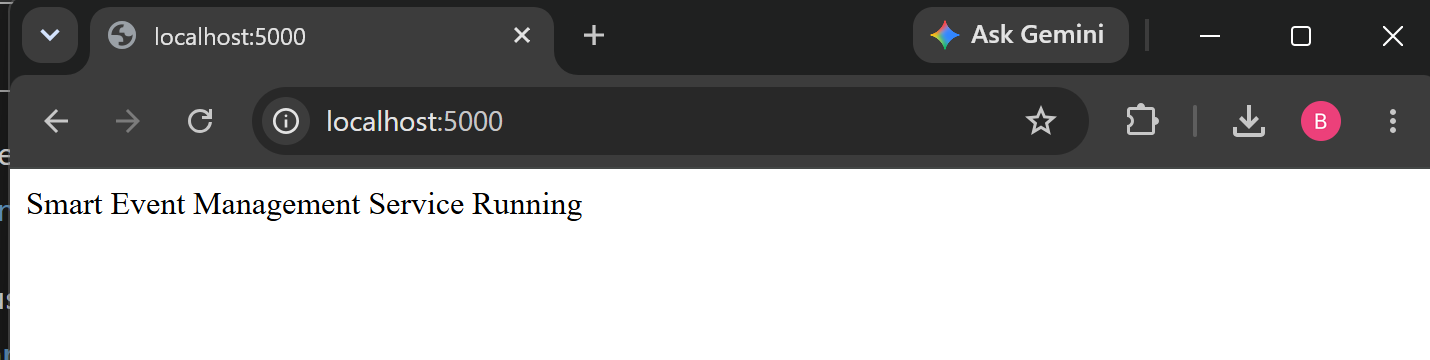
\includegraphics[width=0.85\linewidth]{docker_result.png}}
  \caption{Smart Event Management service running in the Docker container}
  \label{fig:docker}
\end{figure}
To stop the container, press Ctrl+C in the terminal.

% ---------------------------------------------------------------------
\labpart{Reflection Questions}
\question{1. Why is prioritization critical in software projects?}
\answer{Prioritization helps the team finish the most important features with the available time and resources.}
\question{2. How does backlog management help project managers?}
\answer{A backlog keeps all planned work organized and makes it easier to see what should be done next.}
\question{3. How can poor planning affect system architecture later?}
\answer{Poor planning can lead to rushed design choices, messy code, and expensive changes later.}
\question{4. Which part of this lab reflects real industry practice the most?}
\answer{Sprint planning and risk management feel closest to real industry practice because teams use them to organize work and handle problems early.}

% ---------------------------------------------------------------------
\labpart{Expected Deliverables}
Each group must submit:
\begin{itemize}
\item Identified requirements
\item User stories
\item Prioritized backlog
\item Task breakdown
\item Sprint plan
\item Risk table
\item Milestone plan
\item Screenshot of the running Docker container showing the service message in the browser
\end{itemize}

\end{document}
